\chapter[Means for Controlling Animal Inheritance]{The Means Available for Controlling Animal Inheritance}
\label{cha:controlling-animal-inheritance}
\index{Assortive mating|(}
\index{Breeding systems for varied purposes|(}
\index{Inbreeding|(}
\index{Outbreeding|(}
\index{Random mating|(}
\index{Selection|(}

Man can do only a few kinds of things to change the heredity of his
animals. First of all he has some power to decide which of them shall
have many offspring, which shall have few and which shall have none.
That is selection. Selection has always been practiced by animal breeders,
and among many of them it is almost the only breeding method
used. There can be various degrees of it. It can be based on individuality,
on ancestry, on progeny, or on combinations of those in different
degrees.

In the second place, since those chosen to be parents will not be
exactly alike, either in pedigree or in their own somatic appearance and
performance, there are many different ways in which the breeder may
decide which of the chosen males are to be mated to which of the chosen
females. But in their genetic nature and practical consequences all
these systems of mating, if they deviate at all from random mating within
the group of chosen parents, may be classified as the mating of like to
like or as the mating of unlikes. Likeness or unlikeness may be based
either on blood relationship or on individual appearance and performance.

Mating systems, wherein the mates have a closer blood relationship
to each other than if mating were at random, are \textit{inbreeding} in the
broad sense of that word, although most animal breeders reserve that
term for the closest degrees of inbreeding. Mating systems wherein the
mates are less closely related to each other by blood than they would be
under random mating are \textit{outbreeding}. The consequences and uses of
inbreeding and outbreeding were but vaguely known in pre-Mendelian
days. Inbreeding and outbreeding are still used only a little by most
breeders of purebreds; but now that the reasons for their results are
understood and measures of their intensity have been found, considerable
increase in their use seems likely in the future. The results of mating
like to like\index{Mating like to like} or of mating unlikes\index{Mating unlikes} on the basis of their own individual
characteristics, regardless of pedigree, are very different from the results
of inbreeding and outbreeding. Since selection and these four general
systems of mating are the only tools with which man can change the
inheritance of his animals, it is important for the practical breeder to
know what kind of change each is apt to produce, what things each will
do well and what each will do poorly or not at all, what are the chief
dangers or difficulties in each, and what are the most useful means of
overcoming those dangers and difficulties.

Any of these four kinds of mating systems can be practiced in combination
with or in alternation with any of the others. They are almost
always accompanied by some degree of selection. That makes possible
an almost infinite number of specific breeding plans. The probable consequences
of each of those may be predicted in a general way, but the
chance involved in Mendelian segregation and recombination will
leave room for surprising results in individual cases. Moreover, the
combination of one mating system with another will sometimes give
results which are not simply the sum of what each would accomplish if
practiced separately --- an epistatic effect among the breeding systems
themselves, so to speak! There is no immediate prospect that reliable
predictions of the outcome of breeding plans can become so detailed
and accurate that they will remove from the business of livestock
breeding the sporting element of hope and uncertainty which has
been one of its great attractions and has led many wealthy men to take
it up as a hobby.

Man's knowledge of how the mechanism of inheritance operates is
fairly complete, but that knowledge has not yet given him any ability to
interfere with some of the processes so as to change their outcome in the
direction he wishes. Thus, no way has yet been found to control the
segregation of genes so as to produce from heterozygous parents gametes
which contain more than a random proportion of the desired genes.
Nor is there any prospect that such control over assortment at segregation
will ever be achieved. All that man can yet do in this respect is to
select from among those animals available for parents the ones which
suit him best and then accept whatever gametes they produce. But even
after the gametes are produced, he cannot select those which most nearly
have the genes\footnote{P. C. Mangelsdorf has shown (1931, \textit{Proc.
Nat. Acad. Sci.}, 17:698-700) that it is physically possible by the use of
certain mechanical sieving methods to separate com pollen grams which carry
the gene for ``sugary'' from those pollen grains which carry the allelic gene
for ``starchy,'' but the method has not found practical application. Several
attempts to separate male-producing from female-producing spermatozoa by
physical or chemical methods have been tried without success.} he prefers or
promote the union of those which are most like each other or least like each
other. All he can do is to let the array of gametes from the chosen sire unite
at random with whatever ova the chosen dam has produced. There is extensive evidence from
plants that selective fertilization\index{Selective fertilization} exists in nature,\footnote{Jones, D. F. 1928.
\textit{Selective Fertilization}. 163 pp. University of Chicago Press.} but the general
importance of this is in some doubt. In the mildest forms of selective
fertilization in plants, pollen tubes containing genes like those in the
tissue of the plant being fertilized grow down the style toward the
ovule a little faster (or a little more slowly) than pollen tubes which
carry unlike genes. This gives some kinds of genes an advantage over
others in reaching the ovule and fertilizing it, although the handicapped
genes are perfectly capable of doing so if they have no competition
from the favored genes. Whether there is anything to correspond to
this in the higher animals is uncertain, although the processes of animal
courtship may possibly indicate that there is considerable assortive
mating in nature.\footnote{For a summary of knowledge concerning that in Drosophila, see \textit{Biological
Symposia} 6:277--79. 1942.} The most extreme forms of selective fertilization in
plants are cross-sterility or self-sterility, which are phenomena well known
among certain horticultural crops such as some varieties of
apples. Definite genes for self-sterility, often long series of multiple
alleles, are well known in some cases (\textit{Genetics} 27:333--38. 1942). Occasionally
it happens with animals that a female is bred several times to
one male without conceiving but conceives promptly when bred to
another male, although the first male was fertile in matings with other
females. Yet such cases rarely furnish any very plausible indication of
selective fertility since one cannot know whether that female would
have conceived if she had been bred again that last time to the first sire.
There are almost never enough such cases at any one time for a statistical
investigation to be decisive.

Neither can the breeder change the laws of Mendelism nor the number
of genes nor their linkage relations. He cannot change their mutual
physiological interactions, such as dominance, except as he can find and
increase the frequency of other genes which modify in the desired way
the physiological effects of the first genes. To a very limited extent
genes can be changed into other kinds by such violent treatments as
exposure to X-rays, radium, etc.; but such treatments usually result in
a high degree of sterility in the treated animals, and the mutations produced
are so nearly all undesirable\footnote{Gowen and Gay found in their material
(\textit{Genetics} 18:1--31) that 92.2 per cent of all mutations were actually
lethal and many of the rest obviously caused low viability.} that the production
of mutations offers no help to the practical breeder.

This leaves as the breeder's only practical means of controlling the
heredity of his animals his partial freedom to decide how many offspring
each animal shall have and his freedom to choose, within the
group selected for breeding, which shall be mated with which. These
opportunities the breeder possessed and used before Mendel's work was
known. But he used them with many mistakes, and he neglected many
opportunities to use mating systems which could have forwarded his
work. Full use of the genetic knowledge available today should make
the mistakes in selection fewer, although it cannot prevent them all,
and should enable freer use of inbreeding\index{Inbreeding}, outbreeding, and the crossing
of types than breeders would have dared before the principles
underlying those practices were understood.\index{Assortive mating|)}
Perhaps the analogy is not
too fanciful if we compare pre-Mendelian animal breeding with the
animal breeding now possible in the same way we would compare the
common practice of making soap on farms less than a century ago with
the processes now used in modern soap factories. The fundamental
chemistry of soapmaking has not changed; but the product has changed
tremendously in variety, usefulness, adaptability and dependability, as
a result of accumulated refinements in the purity of the ingredients,
closer control of temperatures and concentrations and the use of small
amounts of certain ingredients whose effects were formerly but dimly
understood.

\begin{figure}[htbp]
	\centering
    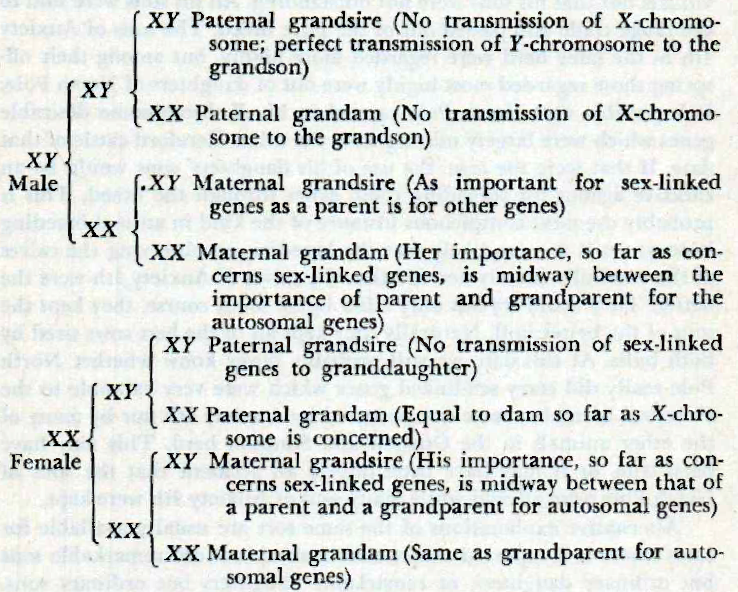
\includegraphics[width=\textwidth]{Page_353.png}
    \label{fig:Lush_Page_353}
    \index{Inbreeding|)}
    \index{Mating like to like}
    \index{Mating unlikes}
    \index{Outbreeding|)}
    \index{Random mating|)}
    \index{Selection|)}
\end{figure}

The above classification may make clearer the kinds and definitions of breeding systems.
\index{Breeding systems for varied purposes|)}